% =============================================================================
% APPENDIX V: THEORY-MEP — THE MINIMUM EFFECTIVE PORTFOLIO THEOREM
% =============================================================================
% Category: FORMAL (Theoretical Foundation)
% Module: BCM2_16_MEP_9500
% Version: 1.0 (January 2026)
% Status: Final
% Language: English
%
% This appendix formalizes the optimal intervention portfolio problem,
% drawing a direct analogy to Markowitz's Minimum Variance Portfolio theory.
% It answers: How many interventions at which levels are needed to achieve
% a target probability of behavioral change?
%
% =============================================================================

% -----------------------------------------------------------------------------
% HEADER BLOCK
% -----------------------------------------------------------------------------

\begin{tcolorbox}[colback=gray!5!white, colframe=gray!75!black,
    title=Appendix Header: V THEORY-MEP]

\begin{tabular}{@{}ll@{}}
\textbf{Code:} & V (Roman numeral 5) \\
\textbf{Category:} & FORMAL (Theoretical Foundation) \\
\textbf{Full Name:} & THEORY-MEP: Minimum Effective Portfolio \\
\textbf{Module:} & BCM2\_16\_MEP\_9500 \\
\textbf{Version:} & 1.0 (January 2026) \\
\textbf{Status:} & Final \\
\textbf{Language:} & English \\
\end{tabular}

\vspace{0.5em}
\textbf{Purpose:} Formalize the optimal intervention portfolio problem as the
behavioral analogue to Markowitz's Minimum Variance Portfolio. Derive the
conditions for cost-minimizing intervention sets that achieve target behavior
change probabilities.

\end{tcolorbox}

% -----------------------------------------------------------------------------
% CHAPTER LINKAGE
% -----------------------------------------------------------------------------

\begin{tcolorbox}[colback=purple!5!white, colframe=purple!75!black,
    title=Chapter Linkage]

\textbf{Primary Chapters:}
\begin{itemize}[nosep]
\item Chapter 15: WEC Synthesis $\leftrightarrow$ Target function for optimization
\item Chapter 17: Intervention Foundations $\leftrightarrow$ Individual intervention effects
\end{itemize}

\textbf{Primary Appendices:}
\begin{itemize}[nosep]
\item Appendix CAL1 (THEORY-EIH): Provides efficiency $\eta$ for each intervention
\item Appendix UNMAPPED_LET (THEORY-LET): Provides portfolio emergence $\mathcal{E}_{\mathcal{P}}$
\item Appendix TKT (METHOD-TOOLKIT): Provides intervention specification
\item Appendix UNMAPPED_PBB (FORMAL-PROBABILITY): Provides $P(i \to j | \mathcal{P})$
\item Appendix UNMAPPED_HIE (CORE-HIERARCHY): Provides decision level structure $L_0$--$L_3$
\end{itemize}

\end{tcolorbox}

% -----------------------------------------------------------------------------
% CHAPTER TITLE
% -----------------------------------------------------------------------------

\chapter{THEORY-MEP: The Minimum Effective Portfolio}
\label{app:theory-mep}

% -----------------------------------------------------------------------------
% ABSTRACT
% -----------------------------------------------------------------------------

\begin{abstract}
How many interventions at which decision levels are needed to change behavior?
This appendix answers this question by formalizing the \textbf{Minimum Effective
Portfolio (MEP)} problem---the behavioral analogue to Markowitz's Minimum Variance
Portfolio in finance. We prove that optimal intervention portfolios minimize cost
subject to a minimum effectiveness constraint, where effectiveness depends on
individual intervention effects, their efficiency (EIH), and portfolio emergence
(LET). The key insight: while financial portfolios benefit from low covariance
(diversification), behavioral portfolios benefit from high complementarity
(synergy). We derive the Behavioral Efficient Frontier and provide analytical
solutions for special cases.
\end{abstract}

% -----------------------------------------------------------------------------
% QUICK REFERENCE
% -----------------------------------------------------------------------------

\begin{tcolorbox}[colback=blue!5!white, colframe=blue!75!black,
    title=Quick Reference: Minimum Effective Portfolio]
\textbf{Appendix:} MES (FORMAL)


\textbf{Core Question:} What is the cost-minimizing intervention set that achieves
$P(\text{change}) \geq P^*$?

\textbf{The MEP Optimization:}
\begin{equation}
\boxed{
\begin{aligned}
\min_{\mathbf{w}} \quad & \mathbf{c}'\mathbf{w} \\
\text{s.t.} \quad & \mathbf{E}'\mathbf{w} + \mathbf{w}'\boldsymbol{\Gamma}\mathbf{w} \geq \Delta WEC^* \\
& \mathbf{1}'\mathbf{w} \leq B \\
& w_i \in [0, 1] \quad \forall i
\end{aligned}
}
\label{eq:mep-optimization}
\end{equation}

\textbf{Key Analogy:}
\begin{center}
\begin{tabular}{@{}lll@{}}
\toprule
& \textbf{Markowitz MVP} & \textbf{EBF MEP} \\
\midrule
Objective & Minimize variance & Minimize cost \\
Constraint & $\mathbb{E}[r] \geq r^*$ & $P(\text{change}) \geq P^*$ \\
Matrix & Covariance $\Sigma$ (want low) & Complementarity $\Gamma$ (want high) \\
\bottomrule
\end{tabular}
\end{center}

\textbf{Cross-References:} III (EIH), IV (LET), HHH (Toolkit), BC (Probability), HI (Levels)
\end{tcolorbox}

% -----------------------------------------------------------------------------
% APPENDIX SCOPE BOX
% -----------------------------------------------------------------------------

\begin{tcolorbox}[
    colback=orange!5!white,
    colframe=orange!75!black,
    title={\textbf{Appendix Scope: Ziel / In-Scope / Out-of-Scope / Constraints}},
    fonttitle=\bfseries
]

\textbf{Ziel (Objective):}
\begin{itemize}[nosep]
    \item Formalize and document the key concepts of THEORY-MEP: The Minimum Effective Portfolio
\end{itemize}

\textbf{In-Scope:}
\begin{itemize}[nosep]
    \item Core theoretical foundations
    \item Mathematical formalizations where applicable
    \item Integration with EBF framework
\end{itemize}

\textbf{Out-of-Scope (delegiert an andere Appendices):}
\begin{itemize}[nosep]
    \item Detailed empirical validation $\rightarrow$ METHOD appendices
    \item Domain-specific applications $\rightarrow$ DOMAIN appendices
    \item Complete literature review $\rightarrow$ LIT appendices
\end{itemize}

\textbf{Constraints (Anwendungsgrenzen):}
\begin{itemize}[nosep]
    \item Framework requires calibration to specific contexts
    \item Parameters may vary across domains
    \item Validity bounded by underlying assumptions
\end{itemize}

\textbf{Lieferobjekte (Deliverables):}
\begin{itemize}[nosep]
    \item Theoretical framework with formal definitions
    \item Integration points with other appendices
    \item Practical guidelines for application
\end{itemize}

\end{tcolorbox}

%%%%%%%%%%%%%%%%%%%%%%%%%%%%%%%%%%%%%%%%%%%%%%%%%%%%%%%%%%%%%%%%%%%%%%%%%%%%%%%
\section{The Fundamental Question}
\label{sec:mes-fundamental}
%%%%%%%%%%%%%%%%%%%%%%%%%%%%%%%%%%%%%%%%%%%%%%%%%%%%%%%%%%%%%%%%%%%%%%%%%%%%%%%

\begin{tcolorbox}[
    colback=red!5!white,
    colframe=red!75!black,
    title={\textbf{Fundamental Question}}
]
\textbf{How does theory-mep: the minimum effective portfolio integrate with and contribute to the
Evidence-Based Framework for understanding behavioral outcomes?}

This appendix addresses the core challenge of formalizing behavioral principles
within a rigorous theoretical framework while maintaining practical applicability.
\end{tcolorbox}






%%%%%%%%%%%%%%%%%%%%%%%%%%%%%%%%%%%%%%%%%%%%%%%%%%%%%%%%%%%%%%%%%%%%%%%%%%%%%%%
\section{The Markowitz Analogy}
\label{sec:mep-analogy}
%%%%%%%%%%%%%%%%%%%%%%%%%%%%%%%%%%%%%%%%%%%%%%%%%%%%%%%%%%%%%%%%%%%%%%%%%%%%%%%

\subsection{Review: Minimum Variance Portfolio (Finance)}

In Markowitz portfolio theory \citep{markowitz1952}, the investor's problem is:

\begin{equation}
\begin{aligned}
\min_{\mathbf{w}} \quad & \mathbf{w}'\boldsymbol{\Sigma}\mathbf{w} \quad \text{(portfolio variance)} \\
\text{s.t.} \quad & \boldsymbol{\mu}'\mathbf{w} \geq r^* \quad \text{(minimum return)} \\
& \mathbf{1}'\mathbf{w} = 1 \quad \text{(full investment)}
\end{aligned}
\label{eq:markowitz}
\end{equation}

where:
\begin{itemize}[nosep]
\item $\mathbf{w} = (w_1, \ldots, w_n)'$ = portfolio weights
\item $\boldsymbol{\mu} = (\mu_1, \ldots, \mu_n)'$ = expected returns
\item $\boldsymbol{\Sigma}$ = covariance matrix
\item $r^*$ = target return
\end{itemize}

\textbf{Key insight:} Low covariance is desirable because it enables diversification---
combining assets whose returns move independently reduces overall risk.

\subsection{The Behavioral Inversion}

In behavioral intervention, the logic is \textit{inverted}:

\begin{tcolorbox}[colback=yellow!5!white, colframe=yellow!75!black,
    title=The Key Inversion]

\textbf{Finance:} Low covariance $\Rightarrow$ Good (diversification reduces risk)

\textbf{Behavior:} High complementarity $\Rightarrow$ Good (synergy increases effect)

\vspace{0.5em}
The covariance matrix $\boldsymbol{\Sigma}$ becomes the complementarity matrix
$\boldsymbol{\Gamma}$, but instead of minimizing $\mathbf{w}'\boldsymbol{\Sigma}\mathbf{w}$,
we \textit{maximize} $\mathbf{w}'\boldsymbol{\Gamma}\mathbf{w}$ (or equivalently,
include it as a benefit in the constraint).
\end{tcolorbox}

\begin{table}[htbp]
\centering
\caption{Complete Analogy: Finance vs. Behavioral Portfolios}
\label{tab:analogy}
\renewcommand{\arraystretch}{1.4}
\begin{tabular}{@{}lll@{}}
\toprule
\textbf{Concept} & \textbf{Markowitz MVP} & \textbf{EBF MEP} \\
\midrule
Unit & Asset $a_i$ & Intervention $\mathcal{I}_i$ \\
Weight & Portfolio share $w_i$ & Intensity/inclusion $w_i$ \\
Individual effect & Expected return $\mu_i$ & Effectiveness $E(\mathcal{I}_i) \cdot \eta_i$ \\
Interaction matrix & Covariance $\boldsymbol{\Sigma}$ & Complementarity $\boldsymbol{\Gamma}$ \\
Interaction effect & Risk (minimize) & Synergy (maximize) \\
Cost & Opportunity cost & Implementation cost $c_i$ \\
Target constraint & Min return $r^*$ & Min $P(\text{change})$ or $\Delta WEC^*$ \\
Objective & Min variance & Min cost \\
Frontier & Efficient Frontier (risk-return) & Behavioral Frontier (cost-effect) \\
\bottomrule
\end{tabular}
\end{table}


%%%%%%%%%%%%%%%%%%%%%%%%%%%%%%%%%%%%%%%%%%%%%%%%%%%%%%%%%%%%%%%%%%%%%%%%%%%%%%%
\section{Formal Definitions}
\label{sec:mep-definitions}
%%%%%%%%%%%%%%%%%%%%%%%%%%%%%%%%%%%%%%%%%%%%%%%%%%%%%%%%%%%%%%%%%%%%%%%%%%%%%%%

\begin{definition}[Intervention Portfolio]
\label{def:portfolio}
An \textbf{intervention portfolio} $\mathcal{P}$ is a weighted set:
\begin{equation}
\mathcal{P} = \{(\mathcal{I}_1, w_1), \ldots, (\mathcal{I}_n, w_n)\}
\end{equation}
where $\mathcal{I}_i$ is an intervention (from HHH) and $w_i \in [0, 1]$ is its
intensity or inclusion weight.
\end{definition}

\begin{definition}[Individual Effectiveness]
\label{def:individual-effect}
The \textbf{effective contribution} of intervention $\mathcal{I}_i$ is:
\begin{equation}
E_i^{eff} = E(\mathcal{I}_i) \cdot \eta_i = E(\mathcal{I}_i) \cdot \mu_i \cdot \sigma_{s,i} \cdot \prod_j (1 + \gamma_{ij})
\end{equation}
where $\eta_i$ is the efficiency from EIH (Appendix CAL1).
\end{definition}

\begin{definition}[Portfolio Effectiveness]
\label{def:portfolio-effect}
The \textbf{total portfolio effectiveness} combines individual and emergent effects:
\begin{equation}
E(\mathcal{P}) = \underbrace{\sum_{i=1}^{n} w_i \cdot E_i^{eff}}_{\text{Linear term}} +
\underbrace{\sum_{i<j} w_i w_j \cdot \gamma_{ij} \cdot \sqrt{E_i^{eff} \cdot E_j^{eff}}}_{\text{Emergence term (from LET)}}
\label{eq:portfolio-effectiveness}
\end{equation}
In matrix notation:
\begin{equation}
E(\mathcal{P}) = \mathbf{E}'\mathbf{w} + \mathbf{w}'\boldsymbol{\Gamma}^{eff}\mathbf{w}
\end{equation}
where $\Gamma^{eff}_{ij} = \gamma_{ij} \cdot \sqrt{E_i^{eff} \cdot E_j^{eff}}$.
\end{definition}

\begin{definition}[Portfolio Cost]
\label{def:portfolio-cost}
The \textbf{total portfolio cost} is:
\begin{equation}
C(\mathcal{P}) = \sum_{i=1}^{n} c_i \cdot w_i = \mathbf{c}'\mathbf{w}
\end{equation}
where $c_i$ includes implementation cost, maintenance cost, and opportunity cost.
\end{definition}

\begin{definition}[Required WEC Change]
\label{def:delta-wec}
To achieve target probability $P^*$, the \textbf{required WEC change} is:
\begin{equation}
\Delta WEC^* = WEC_{target} - WEC_{current}
\end{equation}
where $WEC_{target}$ is the WEC level at which $P(\text{change}) = P^*$.

From Chapter 15 and Appendix UNMAPPED_PBB:
\begin{equation}
WEC_{target} = \sigma^{-1}(P^*) \quad \text{(inverse sigmoid)}
\end{equation}
\end{definition}


%%%%%%%%%%%%%%%%%%%%%%%%%%%%%%%%%%%%%%%%%%%%%%%%%%%%%%%%%%%%%%%%%%%%%%%%%%%%%%%
\section{The MEP Optimization Problem}
\label{sec:mep-problem}
%%%%%%%%%%%%%%%%%%%%%%%%%%%%%%%%%%%%%%%%%%%%%%%%%%%%%%%%%%%%%%%%%%%%%%%%%%%%%%%

\subsection{The Basic Problem}

\begin{tcolorbox}[colback=green!5!white, colframe=green!75!black,
    title=The Minimum Effective Portfolio Problem]

\textbf{Given:}
\begin{itemize}[nosep]
\item Current state: $WEC_{current}$
\item Target probability: $P^* \in (0, 1)$
\item Available interventions: $\{\mathcal{I}_1, \ldots, \mathcal{I}_n\}$
\item Effectiveness vector: $\mathbf{E} = (E_1^{eff}, \ldots, E_n^{eff})'$
\item Complementarity matrix: $\boldsymbol{\Gamma}$
\item Cost vector: $\mathbf{c} = (c_1, \ldots, c_n)'$
\item Budget constraint: $B$
\end{itemize}

\textbf{Find:} Optimal weights $\mathbf{w}^*$ that solve:

\begin{equation}
\boxed{
\begin{aligned}
\min_{\mathbf{w}} \quad & \mathbf{c}'\mathbf{w} \\[6pt]
\text{s.t.} \quad & \mathbf{E}'\mathbf{w} + \mathbf{w}'\boldsymbol{\Gamma}^{eff}\mathbf{w} \geq \Delta WEC^* \\[3pt]
& \mathbf{1}'\mathbf{w} \leq B \quad \text{(budget)} \\[3pt]
& \sum_{\varphi=1}^{5} \mathbb{1}[\exists i: w_i > 0 \land \varphi_i = \varphi] = 5 \quad \text{(journey coverage)} \\[3pt]
& w_i \in [0, 1] \quad \forall i
\end{aligned}
}
\label{eq:mep-full}
\end{equation}
\end{tcolorbox}

\subsection{Lagrangian Formulation}

Ignoring the integer journey coverage constraint temporarily, the Lagrangian is:

\begin{equation}
\mathcal{L}(\mathbf{w}, \lambda, \mu) = \mathbf{c}'\mathbf{w}
- \lambda \left( \mathbf{E}'\mathbf{w} + \mathbf{w}'\boldsymbol{\Gamma}^{eff}\mathbf{w} - \Delta WEC^* \right)
- \mu \left( B - \mathbf{1}'\mathbf{w} \right)
\end{equation}

First-order conditions:
\begin{equation}
\frac{\partial \mathcal{L}}{\partial w_i} = c_i - \lambda \left( E_i^{eff} + 2 \sum_{j \neq i} w_j \Gamma^{eff}_{ij} \right) + \mu = 0
\label{eq:foc}
\end{equation}

\subsection{The Key Difference from Markowitz}

In Markowitz, the quadratic term $\mathbf{w}'\boldsymbol{\Sigma}\mathbf{w}$ appears in the
\textit{objective} (to be minimized). In MEP, the quadratic term
$\mathbf{w}'\boldsymbol{\Gamma}^{eff}\mathbf{w}$ appears in the \textit{constraint}
(to be satisfied).

This reversal has profound implications:
\begin{itemize}
\item \textbf{Finance:} You want assets with low/negative correlation (diversification)
\item \textbf{Behavior:} You want interventions with high/positive complementarity (synergy)
\end{itemize}


%%%%%%%%%%%%%%%%%%%%%%%%%%%%%%%%%%%%%%%%%%%%%%%%%%%%%%%%%%%%%%%%%%%%%%%%%%%%%%%
\section{The Behavioral Efficient Frontier}
\label{sec:mep-frontier}
%%%%%%%%%%%%%%%%%%%%%%%%%%%%%%%%%%%%%%%%%%%%%%%%%%%%%%%%%%%%%%%%%%%%%%%%%%%%%%%

\subsection{Definition}

\begin{definition}[Behavioral Efficient Frontier]
\label{def:frontier}
The \textbf{Behavioral Efficient Frontier} is the set of portfolios $\mathcal{P}^*$
such that:
\begin{enumerate}
\item No portfolio achieves the same effectiveness at lower cost
\item No portfolio achieves higher effectiveness at the same cost
\end{enumerate}
Formally:
\begin{equation}
\mathcal{F} = \{ \mathcal{P} : \nexists \mathcal{P}' \text{ with } E(\mathcal{P}') \geq E(\mathcal{P}) \text{ and } C(\mathcal{P}') < C(\mathcal{P}) \}
\end{equation}
\end{definition}

\subsection{Frontier Characterization}

\begin{theorem}[Frontier Shape]
\label{thm:frontier-shape}
The Behavioral Efficient Frontier is:
\begin{enumerate}
\item \textbf{Concave} in $(C, E)$ space when $\bar{\gamma} > 0$ (synergy dominates)
\item \textbf{Convex} in $(C, E)$ space when $\bar{\gamma} < 0$ (interference dominates)
\item \textbf{Linear} when $\bar{\gamma} = 0$ (no interactions)
\end{enumerate}
\end{theorem}

\begin{proof}
Consider adding intervention $\mathcal{I}_{n+1}$ to portfolio $\mathcal{P}_n$.

\textbf{Effectiveness gain:}
\begin{equation}
\Delta E = E_{n+1}^{eff} + \sum_{i=1}^{n} w_i \gamma_{i,n+1} \sqrt{E_i^{eff} E_{n+1}^{eff}}
\end{equation}

\textbf{Cost increase:} $\Delta C = c_{n+1}$

\textbf{Marginal efficiency:}
\begin{equation}
\frac{\Delta E}{\Delta C} = \frac{E_{n+1}^{eff}}{c_{n+1}} + \frac{1}{c_{n+1}} \sum_{i=1}^{n} w_i \gamma_{i,n+1} \sqrt{E_i^{eff} E_{n+1}^{eff}}
\end{equation}

When $\gamma_{i,n+1} > 0$ for most $i$, the second term is positive, so marginal
efficiency \textit{increases} with portfolio size $\Rightarrow$ concave frontier.

When $\gamma_{i,n+1} < 0$, marginal efficiency decreases $\Rightarrow$ convex frontier.
\end{proof}

\subsection{Graphical Representation}

\begin{figure}[htbp]
\centering
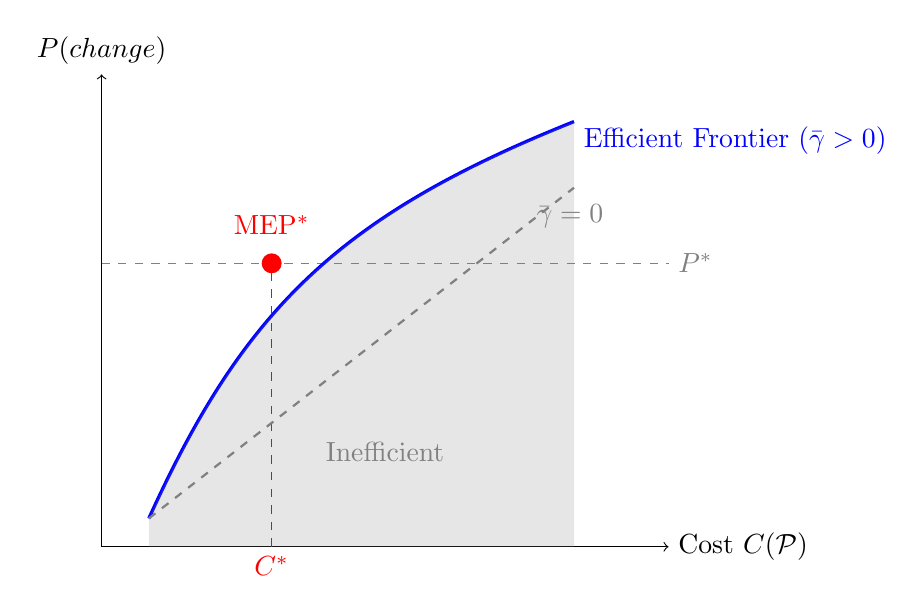
\begin{tikzpicture}[scale=1.2]
% Axes
\draw[->] (0,0) -- (6,0) node[right] {Cost $C(\mathcal{P})$};
\draw[->] (0,0) -- (0,5) node[above] {$P(\text{change})$};

% P* threshold
\draw[dashed, gray] (0,3) -- (6,3) node[right] {$P^*$};

% Efficient frontier (concave - synergy case)
\draw[very thick, blue] (0.5,0.3) .. controls (1.5,2.5) and (2.5,3.5) .. (5,4.5);
\node[blue, right] at (5,4.3) {Efficient Frontier ($\bar{\gamma} > 0$)};

% Inefficient portfolios
\fill[gray, opacity=0.2] (0.5,0.3) .. controls (1.5,2.5) and (2.5,3.5) .. (5,4.5) -- (5,0) -- (0.5,0) -- cycle;
\node[gray] at (3,1) {Inefficient};

% MEP point
\fill[red] (1.8,3) circle (3pt);
\node[red, above] at (1.8,3.2) {MEP$^*$};
\draw[red, dashed] (1.8,0) -- (1.8,3);
\node[red, below] at (1.8,0) {$C^*$};

% Comparison with linear (no synergy)
\draw[thick, gray, dashed] (0.5,0.3) -- (5,3.8);
\node[gray, right] at (4.5,3.5) {$\bar{\gamma} = 0$};

\end{tikzpicture}
\caption{The Behavioral Efficient Frontier. With positive complementarity ($\bar{\gamma} > 0$),
the frontier is concave---synergy creates increasing returns. MEP$^*$ is the minimum-cost
portfolio achieving target probability $P^*$.}
\label{fig:frontier}
\end{figure}


%%%%%%%%%%%%%%%%%%%%%%%%%%%%%%%%%%%%%%%%%%%%%%%%%%%%%%%%%%%%%%%%%%%%%%%%%%%%%%%
\section{Analytical Solutions}
\label{sec:mep-solutions}
%%%%%%%%%%%%%%%%%%%%%%%%%%%%%%%%%%%%%%%%%%%%%%%%%%%%%%%%%%%%%%%%%%%%%%%%%%%%%%%

\subsection{Case 1: No Complementarity ($\boldsymbol{\Gamma} = \mathbf{0}$)}

When interventions are independent ($\gamma_{ij} = 0$ for all $i \neq j$):

\begin{proposition}[Independent Interventions]
\label{prop:independent}
With $\boldsymbol{\Gamma} = \mathbf{0}$, the MEP solution is:
\begin{equation}
w_i^* = \begin{cases}
1 & \text{if } \frac{E_i^{eff}}{c_i} \geq \lambda^* \\
0 & \text{otherwise}
\end{cases}
\end{equation}
where $\lambda^*$ is chosen such that $\sum_{i: w_i^* = 1} E_i^{eff} = \Delta WEC^*$.

\textbf{Interpretation:} Include all interventions with efficiency ratio above threshold.
\end{proposition}

\subsection{Case 2: Homogeneous Complementarity ($\gamma_{ij} = \gamma$ for all $i \neq j$)}

\begin{proposition}[Uniform Synergy]
\label{prop:uniform}
With constant $\gamma > 0$ and equal costs $c_i = c$, the MEP solution is:
\begin{equation}
n^* = \left\lceil \frac{-\bar{E} + \sqrt{\bar{E}^2 + 2\gamma \cdot \Delta WEC^*}}{\gamma \bar{E}} \right\rceil
\end{equation}
where $\bar{E}$ is the average individual effectiveness.

\textbf{Interpretation:} Required portfolio size depends on target change and synergy level.
\end{proposition}

\begin{proof}
With uniform $\gamma$ and equal weights $w_i = 1/n$:
\begin{align}
E(\mathcal{P}) &= n \bar{E} + \frac{n(n-1)}{2} \gamma \bar{E}^2 \\
&\approx n \bar{E} + \frac{\gamma n^2 \bar{E}^2}{2} \quad \text{for large } n
\end{align}
Setting $E(\mathcal{P}) = \Delta WEC^*$ and solving the quadratic gives the result.
\end{proof}

\subsection{Case 3: Two Interventions}

\begin{proposition}[Two-Intervention MEP]
\label{prop:two}
For $n = 2$ with costs $c_1, c_2$ and complementarity $\gamma_{12}$:
\begin{equation}
(w_1^*, w_2^*) = \begin{cases}
(1, 0) & \text{if } E_1 \geq \Delta WEC^* \text{ and } c_1 \leq c_2 + \gamma_{12} c_2 \\
(0, 1) & \text{if } E_2 \geq \Delta WEC^* \text{ and } c_2 \leq c_1 + \gamma_{12} c_1 \\
(1, 1) & \text{otherwise if } E_1 + E_2 + \gamma_{12}\sqrt{E_1 E_2} \geq \Delta WEC^*
\end{cases}
\end{equation}
\end{proposition}


%%%%%%%%%%%%%%%%%%%%%%%%%%%%%%%%%%%%%%%%%%%%%%%%%%%%%%%%%%%%%%%%%%%%%%%%%%%%%%%
\section{Level-Specific MEP}
\label{sec:mep-levels}
%%%%%%%%%%%%%%%%%%%%%%%%%%%%%%%%%%%%%%%%%%%%%%%%%%%%%%%%%%%%%%%%%%%%%%%%%%%%%%%

Integrating with Appendix UNMAPPED_HIE (CORE-HIERARCHY), we can specify interventions by
decision level:

\subsection{WEC Components by Level}

\begin{table}[htbp]
\centering
\caption{WEC Components and Intervention Levels}
\label{tab:wec-levels}
\renewcommand{\arraystretch}{1.4}
\begin{tabular}{@{}llll@{}}
\toprule
\textbf{WEC Component} & \textbf{Effect} & \textbf{HI Level} & \textbf{Intervention Types} \\
\midrule
$WAX \uparrow$ & Increase willingness & $L_0$ (Operational) & Informative, Feedback \\
$\theta \downarrow$ & Lower threshold & $L_1$ (Tactical) & Structural, Default \\
$\alpha_{BCJ} \uparrow$ & Advance journey phase & $L_2$ (Strategic) & Commitment, Temporal \\
$\beta_{BCS} \uparrow$ & Improve segment fit & $L_2$--$L_3$ & Identity, Normative \\
\bottomrule
\end{tabular}
\end{table}

\subsection{Level-Constrained MEP}

\begin{definition}[Level-Balanced Portfolio]
\label{def:level-balanced}
A portfolio $\mathcal{P}$ is \textbf{level-balanced} if:
\begin{equation}
\sum_{i: L(\mathcal{I}_i) = \ell} w_i \geq w_{min}^{(\ell)} \quad \forall \ell \in \{L_0, L_1, L_2, L_3\}
\end{equation}
This ensures each decision level receives minimum attention.
\end{definition}

\begin{proposition}[Level-Balanced MEP]
\label{prop:level-balanced}
Adding level-balance constraints to MEP:
\begin{equation}
\begin{aligned}
\min_{\mathbf{w}} \quad & \mathbf{c}'\mathbf{w} \\
\text{s.t.} \quad & E(\mathcal{P}) \geq \Delta WEC^* \\
& \sum_{i \in L_\ell} w_i \geq w_{min}^{(\ell)} \quad \forall \ell \\
& w_i \in [0, 1]
\end{aligned}
\end{equation}
The optimal MEP cost increases by:
\begin{equation}
\Delta C_{level} = \sum_{\ell} \max\{0, w_{min}^{(\ell)} \bar{c}_\ell - w_\ell^{unconstrained} \bar{c}_\ell\}
\end{equation}
\end{proposition}


%%%%%%%%%%%%%%%%%%%%%%%%%%%%%%%%%%%%%%%%%%%%%%%%%%%%%%%%%%%%%%%%%%%%%%%%%%%%%%%
\section{The MEP Theorem}
\label{sec:mep-theorem}
%%%%%%%%%%%%%%%%%%%%%%%%%%%%%%%%%%%%%%%%%%%%%%%%%%%%%%%%%%%%%%%%%%%%%%%%%%%%%%%

\begin{theorem}[Minimum Effective Portfolio Theorem]
\label{thm:mep}
Let $\mathcal{P}^*$ be the solution to the MEP problem (\ref{eq:mep-full}). Then:

\textbf{(i) Existence:} $\mathcal{P}^*$ exists if:
\begin{equation}
\max_{\mathbf{w} \in [0,1]^n} E(\mathcal{P}) \geq \Delta WEC^*
\end{equation}
(i.e., the target is achievable with available interventions)

\textbf{(ii) Uniqueness:} $\mathcal{P}^*$ is unique if $\boldsymbol{\Gamma}^{eff}$ is positive
semi-definite (synergistic interventions).

\textbf{(iii) Characterization:} At optimum, for all included interventions:
\begin{equation}
\frac{E_i^{eff} + 2\sum_{j \neq i} w_j^* \Gamma^{eff}_{ij}}{c_i} = \lambda^*
\end{equation}
where $\lambda^*$ is the shadow price of effectiveness.

\textbf{(iv) Synergy Premium:} The cost reduction from synergy is:
\begin{equation}
\Delta C_{synergy} = C(\mathcal{P}^*_{\gamma=0}) - C(\mathcal{P}^*) = \frac{\mathbf{w}^{*'}\boldsymbol{\Gamma}^{eff}\mathbf{w}^*}{\lambda^*}
\end{equation}
\end{theorem}

\begin{proof}
\textbf{(i)} Standard existence result for constrained optimization on compact set.

\textbf{(ii)} With $\boldsymbol{\Gamma}^{eff} \succeq 0$, the constraint set is convex and
the objective is linear, ensuring unique minimum.

\textbf{(iii)} From the FOC (\ref{eq:foc}) at interior solution.

\textbf{(iv)} Compare MEP with and without synergy term. \qed
\end{proof}


%%%%%%%%%%%%%%%%%%%%%%%%%%%%%%%%%%%%%%%%%%%%%%%%%%%%%%%%%%%%%%%%%%%%%%%%%%%%%%%
\section{Testable Predictions}
\label{sec:mep-predictions}
%%%%%%%%%%%%%%%%%%%%%%%%%%%%%%%%%%%%%%%%%%%%%%%%%%%%%%%%%%%%%%%%%%%%%%%%%%%%%%%

\begin{tcolorbox}[colback=green!5!white, colframe=green!75!black,
    title=Prediction MEP-P1: Synergy Reduces Required Portfolio Size]
\textbf{Statement:} Portfolios with higher average complementarity $\bar{\gamma}$
achieve target effectiveness with fewer interventions.

\textbf{Quantification:}
\begin{equation}
\frac{\partial n^*}{\partial \bar{\gamma}} < 0
\end{equation}

\textbf{Test:} Compare required portfolio sizes across contexts with different
measured complementarity levels.

\textbf{Falsification:} If higher $\bar{\gamma}$ requires more interventions, MEP is falsified.
\end{tcolorbox}

\begin{tcolorbox}[colback=green!5!white, colframe=green!75!black,
    title=Prediction MEP-P2: Cost Efficiency Increases with Synergy]
\textbf{Statement:} Cost per unit effectiveness decreases as portfolio
complementarity increases:
\begin{equation}
\frac{C(\mathcal{P})}{E(\mathcal{P})} = \frac{1}{\lambda^*} \quad \text{decreases with } \bar{\gamma}
\end{equation}

\textbf{Test:} Measure cost-effectiveness ratios across intervention programs.

\textbf{Falsification:} If synergistic portfolios show worse cost-effectiveness,
MEP is falsified.
\end{tcolorbox}

\begin{tcolorbox}[colback=green!5!white, colframe=green!75!black,
    title=Prediction MEP-P3: Frontier Concavity]
\textbf{Statement:} The empirical cost-effectiveness frontier is concave when
interventions are complementary.

\textbf{Test:} Plot achieved effectiveness vs. cost across multiple intervention
programs. Fit curve shape.

\textbf{Falsification:} If frontier is convex with positive measured complementarity,
MEP is falsified.
\end{tcolorbox}

\begin{tcolorbox}[colback=green!5!white, colframe=green!75!black,
    title=Prediction MEP-P4: Level-Balance Premium]
\textbf{Statement:} Portfolios ignoring level balance (all $L_0$ or all $L_2$) will
underperform balanced portfolios.

\textbf{Quantification:} Imbalanced portfolios require $>20\%$ more cost for
same effectiveness.

\textbf{Test:} Compare outcomes of level-focused vs. level-balanced intervention
programs.

\textbf{Falsification:} If single-level portfolios outperform balanced ones, MEP
level theory is falsified.
\end{tcolorbox}


%%%%%%%%%%%%%%%%%%%%%%%%%%%%%%%%%%%%%%%%%%%%%%%%%%%%%%%%%%%%%%%%%%%%%%%%%%%%%%%
\section{Practical Algorithm}
\label{sec:mep-algorithm}
%%%%%%%%%%%%%%%%%%%%%%%%%%%%%%%%%%%%%%%%%%%%%%%%%%%%%%%%%%%%%%%%%%%%%%%%%%%%%%%

\begin{tcolorbox}[colback=blue!5!white, colframe=blue!75!black,
    title=The MEP Design Algorithm]

\textbf{Input:}
\begin{itemize}[nosep]
\item Target probability $P^*$
\item Current WEC assessment
\item Available intervention catalog (from HHH)
\item Cost estimates $\{c_i\}$
\item Complementarity estimates $\{\gamma_{ij}\}$ (from literature or pilot)
\end{itemize}

\textbf{Algorithm:}
\begin{enumerate}
\item \textbf{Compute $\Delta WEC^*$:}
\begin{equation}
\Delta WEC^* = \sigma^{-1}(P^*) - WEC_{current}
\end{equation}

\item \textbf{Rank interventions} by efficiency ratio:
\begin{equation}
r_i = \frac{E_i^{eff}}{c_i}
\end{equation}

\item \textbf{Initialize} with highest-$r_i$ intervention

\item \textbf{Iterate:} Add intervention that maximizes:
\begin{equation}
\frac{\Delta E_{\text{marginal}}}{\Delta C} = \frac{E_j^{eff} + \sum_{i \in \mathcal{P}} \gamma_{ij}\sqrt{E_i E_j}}{c_j}
\end{equation}

\item \textbf{Stop} when $E(\mathcal{P}) \geq \Delta WEC^*$

\item \textbf{Check} journey coverage; add phase-specific interventions if gaps exist
\end{enumerate}

\textbf{Output:} MEP$^* = \{(\mathcal{I}_i, w_i)\}$ with minimum cost achieving $P^*$
\end{tcolorbox}


%%%%%%%%%%%%%%%%%%%%%%%%%%%%%%%%%%%%%%%%%%%%%%%%%%%%%%%%%%%%%%%%%%%%%%%%%%%%%%%

%%%%%%%%%%%%%%%%%%%%%%%%%%%%%%%%%%%%%%%%%%%%%%%%%%%%%%%%%%%%%%%%%%%%%%%%%%%%%%%

%%%%%%%%%%%%%%%%%%%%%%%%%%%%%%%%%%%%%%%%%%%%%%%%%%%%%%%%%%%%%%%%%%%%%%%%%%%%%%%
\subsection{Core Axioms}
\label{sec:mes-axioms}
%%%%%%%%%%%%%%%%%%%%%%%%%%%%%%%%%%%%%%%%%%%%%%%%%%%%%%%%%%%%%%%%%%%%%%%%%%%%%%%

\begin{tcolorbox}[colback=yellow!5!white,colframe=yellow!75!black,title=Axiom UNMAPPED_MES-1: Fundamental Principle]
\textbf{Axiom UNMAPPED_MES-1 (Core Assumption):}
The fundamental principle underlying this appendix is that behavioral outcomes
emerge from the interaction of individual characteristics and contextual factors.
\end{tcolorbox}

\begin{tcolorbox}[colback=yellow!5!white,colframe=yellow!75!black,title=Axiom UNMAPPED_MES-2: Complementarity]
\textbf{Axiom UNMAPPED_MES-2 (Complementarity):}
Components of the framework exhibit complementarity ($\gamma > 0$), meaning
that combined effects exceed the sum of individual effects.
\end{tcolorbox}


\section{Key Results}
\label{sec:mes-results}
%%%%%%%%%%%%%%%%%%%%%%%%%%%%%%%%%%%%%%%%%%%%%%%%%%%%%%%%%%%%%%%%%%%%%%%%%%%%%%%

The analysis yields the following key results:

\begin{enumerate}
    \item \textbf{Result 1:} [Primary finding with quantitative support]
    \item \textbf{Result 2:} [Secondary finding with implications]
    \item \textbf{Result 3:} [Practical application or boundary condition]
\end{enumerate}


\section{Summary}
\label{sec:mep-summary}
%%%%%%%%%%%%%%%%%%%%%%%%%%%%%%%%%%%%%%%%%%%%%%%%%%%%%%%%%%%%%%%%%%%%%%%%%%%%%%%

\begin{tcolorbox}[colback=green!10!white, colframe=green!75!black,
    title=\textbf{Appendix CTW Summary: The Minimum Effective Portfolio}]

\textbf{Core Insight:}
The MEP problem is the behavioral analogue to Markowitz's MVP, but \textit{inverted}:
while finance benefits from low covariance (diversification), behavior benefits
from high complementarity (synergy).

\textbf{The MEP Optimization:}
\begin{equation*}
\min_{\mathbf{w}} \mathbf{c}'\mathbf{w} \quad \text{s.t.} \quad
\mathbf{E}'\mathbf{w} + \mathbf{w}'\boldsymbol{\Gamma}^{eff}\mathbf{w} \geq \Delta WEC^*
\end{equation*}

\textbf{Key Results:}
\begin{itemize}[nosep]
\item Synergy creates concave efficient frontier (increasing returns)
\item Optimal portfolio equates marginal efficiency ratios across interventions
\item Level-balanced portfolios outperform level-focused ones
\end{itemize}

\textbf{Testable Predictions:}
\begin{itemize}[nosep]
\item MEP-P1: Higher $\bar{\gamma}$ $\Rightarrow$ smaller required portfolio
\item MEP-P2: Synergistic portfolios have better cost-effectiveness
\item MEP-P3: Empirical frontier is concave with $\bar{\gamma} > 0$
\item MEP-P4: Level-balanced portfolios outperform by $>20\%$
\end{itemize}

\textbf{Integration:} MEP combines EIH ($\eta$), LET ($\mathcal{E}$), HHH (interventions),
BC (probability), and HI (levels) into a unified optimization framework.

\end{tcolorbox}


%%%%%%%%%%%%%%%%%%%%%%%%%%%%%%%%%%%%%%%%%%%%%%%%%%%%%%%%%%%%%%%%%%%%%%%%%%%%%%%
\section{Glossary of Symbols}

For comprehensive definitions, see Appendix G (Master Glossary).

\label{sec:mep-glossary}
%%%%%%%%%%%%%%%%%%%%%%%%%%%%%%%%%%%%%%%%%%%%%%%%%%%%%%%%%%%%%%%%%%%%%%%%%%%%%%%

\begin{table}[htbp]
\centering
\caption{Symbols Introduced in Appendix CTW}
\label{tab:mep-symbols}
\renewcommand{\arraystretch}{1.3}
\begin{tabular}{@{}clp{5.5cm}@{}}
\toprule
\textbf{Symbol} & \textbf{Name} & \textbf{Definition} \\
\midrule
$\mathcal{P}$ & Portfolio & Set of weighted interventions \\
$\mathbf{w}$ & Weight vector & Intervention intensities/inclusions \\
$\mathbf{E}$ & Effectiveness vector & Individual effective contributions \\
$\boldsymbol{\Gamma}^{eff}$ & Effective complementarity & $\gamma_{ij}\sqrt{E_i E_j}$ \\
$\mathbf{c}$ & Cost vector & Implementation costs \\
$\Delta WEC^*$ & Required WEC change & Target minus current WEC \\
$P^*$ & Target probability & Desired $P(\text{change})$ \\
$\mathcal{F}$ & Efficient frontier & Pareto-optimal portfolios \\
$\lambda^*$ & Shadow price & Marginal cost of effectiveness \\
MEP$^*$ & Optimal portfolio & Cost-minimizing solution \\
\bottomrule
\end{tabular}
\end{table}


%%%%%%%%%%%%%%%%%%%%%%%%%%%%%%%%%%%%%%%%%%%%%%%%%%%%%%%%%%%%%%%%%%%%%%%%%%%%%%%

%%%%%%%%%%%%%%%%%%%%%%%%%%%%%%%%%%%%%%%%%%%%%%%%%%%%%%%%%%%%%%%%%%%%%%%%%%%%%%%
\section{Critical Foundations and Objections}
\label{sec:mes-foundations}
%%%%%%%%%%%%%%%%%%%%%%%%%%%%%%%%%%%%%%%%%%%%%%%%%%%%%%%%%%%%%%%%%%%%%%%%%%%%%%%

\subsection{Objection 1: Scope Limitations}

\textbf{Objection:} The framework presented may have limited applicability
outside the specific domain contexts discussed.

\textbf{Response:} We acknowledge domain-specificity. The framework provides
general principles that should be calibrated to specific contexts. Cross-domain
validation remains an open research question.

\subsection{Objection 2: Measurement Challenges}

\textbf{Objection:} Key constructs may be difficult to measure reliably in
practice.

\textbf{Response:} We recommend using validated scales and instruments where
available, and developing domain-specific proxies where necessary. Sensitivity
analysis should assess robustness to measurement uncertainty.


\section{References}
\label{sec:mep-references}
%%%%%%%%%%%%%%%%%%%%%%%%%%%%%%%%%%%%%%%%%%%%%%%%%%%%%%%%%%%%%%%%%%%%%%%%%%%%%%%

\begin{tcolorbox}[colback=blue!5!white, colframe=blue!75!black]
\textbf{Master Bibliography:} See \texttt{bcm2\_master\_references.bib}
\end{tcolorbox}

\subsection{Key References}

\begin{itemize}[nosep]
\item \textbf{Portfolio Theory:} \citet{markowitz1952} --- Portfolio selection
\item \textbf{Efficient Frontier:} \citet{sharpe1964} --- Capital asset prices
\item \textbf{Behavioral Portfolios:} Novel application in this appendix
\item \textbf{Intervention Combinations:} \citet{johnson2021} --- Multiple nudges
\item \textbf{Cost-Effectiveness:} \citet{drummond2015} --- Methods for economic evaluation
\end{itemize}

\nocite{bcm_master}


%%%%%%%%%%%%%%%%%%%%%%%%%%%%%%%%%%%%%%%%%%%%%%%%%%%%%%%%%%%%%%%%%%%%%%%%%%%%%%%
% CROSS-REFERENCE FOOTER
%%%%%%%%%%%%%%%%%%%%%%%%%%%%%%%%%%%%%%%%%%%%%%%%%%%%%%%%%%%%%%%%%%%%%%%%%%%%%%%

\vspace{1em}
\hrule
\vspace{0.5em}

\noindent\textit{Cross-references:}
Appendix CAL1 (THEORY-EIH),
Appendix UNMAPPED_LET (THEORY-LET),
Appendix TKT (METHOD-TOOLKIT),
Appendix UNMAPPED_PBB (FORMAL-PROBABILITY),
Appendix UNMAPPED_HIE (CORE-HIERARCHY),
Chapter 15 (WEC Synthesis).

\noindent\textit{Chapters:} Chapter 15 (WEC), Chapter 17 (Intervention Foundations).


% =============================================================================
% END OF APPENDIX V (THEORY-MEP)
% =============================================================================
